\documentclass[aps,prd,10pt,nofootinbib,twocolumn,superscriptaddress,floatfix,notitlepage]{revtex4-1}
\usepackage{graphicx}
\usepackage{amsmath,amsfonts,amssymb}
\usepackage{color}
\usepackage[breaklinks,colorlinks,urlcolor=blue,citecolor=blue,linkcolor=magenta]{hyperref}
\usepackage{verbatim}
\usepackage{enumitem}
\usepackage{aas_macros}
\usepackage{tikz}
\newcommand{\Msun}{M_\odot}
\newcommand{\td}{{\rm d}}
\newcommand{\vect}[1]{\boldsymbol{#1}}
\DeclareMathOperator{\artanh}{artanh}
\DeclareMathOperator{\arcoth}{arcoth}
\newcommand{\be}{\begin{equation}}
\newcommand{\ee}{\end{equation}}
\newcommand{\bea}{\begin{equation} \begin{aligned}}
\newcommand{\eea}{\end{aligned} \end{equation}}
\newcommand{\Gala}[1]{{\color{orange} (#1 -- Gala)}}
\def\lsim{\mathrel{\raise.3ex\hbox{$<$\kern-.75em\lower1ex\hbox{$\sim$}}}}
\def\gsim{\mathrel{\raise.3ex\hbox{$>$\kern-.75em\lower1ex\hbox{$\sim$}}}}
\newcommand{\R}[1]{{\color{red} #1}}
\newcommand{\B}[1]{{\color{blue} #1}}

\begin{document}

\title{Learning weak lensing magnifications}

\author{Galymzhan Baltabay}
\email{galymzhan.baltabay@kbfi.ee}
\affiliation{Laboratory of High Energy and Computational Physics, KBFI, R{\"a}vala 10, Tallinn, 10143, Estonia}
\affiliation{Department of Cybernetics, Tallinn University of Technology, Akadeemia tee 21, 12618 Tallinn, Estonia}

\author{Ville Vaskonen}
\email{ville.vaskonen@kbfi.ee}
\affiliation{Laboratory of High Energy and Computational Physics, KBFI, R{\"a}vala 10, Tallinn, 10143, Estonia}

\begin{abstract}
\B{Gravitational-wave standard sirens provide direct, calibration-free measurements of the luminosity distance, and the scatter that weak lensing by intervening structure induces around the mean Hubble diagram is itself a probe of cosmic structure, complementary to the mean distance-redshift relation~\cite{Vaskonen:2026ubd}. Predicting the resulting magnification probability distribution $dP/d\mu$ accurately, however, requires summing the lensing contribution of a large, stochastically realized population of halos, filaments, and their substructure, a computation too slow to repeat at every point of a cosmological parameter scan. We extend the stochastic lensing model of Ref.~\cite{Vaskonen:2026ubd} by adding the contribution of dark matter subhalos and by replacing its independent (Poisson) halo and filament counts with a correlated treatment of large-scale clustering, and we train a conditional normalizing-flow emulator that reproduces the resulting $dP/d\mu$ as a function of the source redshift and the full six-dimensional set of cosmological parameters $\vect\Theta = \{h,\Omega_M,\Omega_B,A_s,n_s,z_{\rm eq}\}$. The emulator matches the simulator to a median Kullback-Leibler divergence of $0.0073$, comparable to existing machine-learning emulators of the magnification distribution, while running orders of magnitude faster than the underlying Monte Carlo, making likelihood-based cosmological inference with the extended lens model computationally practical.}
\end{abstract}

\maketitle

\section{Introduction}

\B{Gravitational waves (GWs) from compact binary mergers with an identified electromagnetic (EM) counterpart are standard sirens, whose luminosity distance is read directly off the waveform amplitude without a distance-ladder calibration. Ref.~\cite{Vaskonen:2026ubd} showed that the scatter weak gravitational lensing induces around the mean luminosity distance-redshift relation is itself sensitive to the amplitude of matter fluctuations, $\sigma_8$, complementing the standard-siren measurement of the Hubble constant $H_0$ and the matter abundance $\Omega_M$. A population of $\mathcal{O}(100)$ bright sirens from third-generation detectors could reach a competitive measurement of $\sigma_8$ this way.}

\B{Exploiting this scatter for cosmological inference requires an accurate model of the magnification probability distribution $dP/d\mu$. One route is ray tracing through the density field of cosmological $N$-body simulations~\cite{Holz:1997ic,Holz:2004xx,Takahashi:2011qd,Takahashi:2017hjr}. Such simulations, however, lack the mass resolution to populate the high-magnification tail of $dP/d\mu$, which is generated by rare, compact structures close to the line of sight~\cite{DES:2025omh}. The stochastic approach of Refs.~\cite{Kainulainen:2009dw,Kainulainen:2010at,Kainulainen:2011zx}, implemented for bright sirens in Ref.~\cite{Vaskonen:2026ubd}, instead builds $dP/d\mu$ by directly summing the contributions of a Monte Carlo-realized population of discrete lenses, resolving magnifications that $N$-body ray tracing misses at a fraction of the computational cost. Even so, evaluating $dP/d\mu$ at the many points of a cosmological parameter space required for Markov chain Monte Carlo inference remains expensive, since each evaluation requires a fresh Monte Carlo realization of the lens population. This has motivated machine-learning emulators of the magnification distribution, such as ACE-Lensing~\cite{Turker:2025rdt}, which learn a fast, differentiable surrogate for $dP/d\mu$ directly from simulated samples.}

\B{In this work we extend the stochastic lensing model of Ref.~\cite{Vaskonen:2026ubd} in two ways. First, we add the previously unmodeled contribution of dark matter subhalos, sampling the substructure of every lensing halo down to a fixed mass floor and subtracting the corresponding mass from the smooth halo profile so that the total halo mass is conserved in every realization. Second, we replace the independent Poisson realization of halo and filament counts with a physically motivated treatment of their large-scale clustering, correlating the lens population along the line of sight with a stochastic realization of the underlying density field, together with the sub-threshold background contribution. We then train a conditional normalizing-flow emulator that reproduces the resulting $dP/d\mu$ as a function of the source redshift $z_s$ and the cosmological parameters $\vect\Theta = \{h,\Omega_M,\Omega_B,A_s,n_s,z_{\rm eq}\}$, matching the fidelity of existing emulators while incorporating this extended physical model.}

\B{The remainder of this paper is organized as follows. In Sec.~\ref{sec:lensing} we describe the stochastic lensing model, including the clustering of field halos, the subhalo contribution, and the resulting magnification distribution. In Sec.~\ref{sec:ml} we describe the emulator and its training. In Sec.~\ref{sec:comparison} we compare our model and its emulator with earlier work. We conclude in Sec.~\ref{sec:conclusions}.}

\section{Weak lensing}
\label{sec:lensing}

\B{Weak gravitational lensing by structures near the line of sight magnifies the observed signal by a factor $\mu$.} Accordingly, the apparent luminosity distance is given by
\be
    D_L(z) = \frac{\tilde{D}_L(z)}{\sqrt{\mu}} \,,
\ee
where $\tilde{D}_L(z)$ denotes the luminosity distance-redshift relation in a homogeneous and isotropic universe.

In the following we briefly describe the stochastic approach that we use for the computation of the distribution of weak lensing magnifications, focusing on how we extend the lens modeling by including DM subhalos.

\subsection{Stochastic approach}

The lensing magnification is given by
\be \label{eq:mueq}
	\mu = \frac{1}{(1-\kappa)^2 - \gamma^2} \,\B{,}
\ee
where the convergence $\kappa$ and the shear $\gamma = \sqrt{\gamma_1^2+\gamma_2^2}$ are, in the weak-lensing approximation, obtained by summing the contributions of individual lenses, $\kappa = \sum_j \kappa_\epsilon(\vect\theta_j)$, $\gamma_1 = \sum_j \gamma_\epsilon(\vect\theta_j) \cos\phi_j$ and $\gamma_2 = \sum_j \gamma_\epsilon(\vect\theta_j) \sin\phi_j$. Here $\phi_j$ denotes the polar angle of the lens position in the lens plane, defined with respect to a coordinate system common to all lenses, and $\vect\theta_j$ encodes the lens redshift $z_j$, its projected distance $r_j$ from line-of-sight to the source, and parameters describing the lens properties and orientation. \B{The subscript $\epsilon$ indicates that $\kappa_\epsilon$ and $\gamma_\epsilon$ are the convergence and shear profiles of the pseudo-elliptically distorted lens models specified below, with $\epsilon$ the ellipticity of the projected profile.}

We include lensing contributions from field halos, subhalos, and filaments. The field halos and filaments are modeled as in~\cite{Vaskonen:2026ubd}. The new ingredient included in this study is the contribution of subhalos. Furthermore, we introduce an improved treatment of the clustering of field halos.

\subsubsection{Clustering}

Long-wavelength linear density perturbations modulate the spatial distribution of halos. The resulting change in the halo number density is governed by the halo bias $b(M,z)$, which increases with halo mass $M$ because massive halos originate from increasingly rare peaks of the primordial density field.

We estimate the halo clustering using the one-dimensional density field $\delta_{\rm 1D}(z) \equiv \delta_{\rm 1D}(d_c(z))$, obtained by smoothing the three-dimensional density field \B{isotropically with a spherical window of comoving radius $R_s$} before projecting onto the line of sight. Its power spectrum is\footnote{This generalizes the pencil-beam construction of Ref.~\cite{1991ApJ...379..482K}, whose $P_{\rm 1D}(k_\parallel)=\int_{k_\parallel}^\infty \td k\,k\,P(k)/(2\pi)$ is recovered in the $R_s\to0$ limit.}
\be
    P_{\rm 1D}(k_\parallel) = \frac{1}{2\pi} \int_{k_\parallel}^\infty \!\td k \, k \, P(k)\, \tilde{W}^2(R_s k) \,,
\ee
\B{where the integration variable is the modulus $k = |\vect{k}|$ and $\tilde{W}(x) = 3(\sin x - x\cos x)/x^3$ is the Fourier transform of the spherical top-hat.} The smoothing suppresses the contribution of scales smaller than $R_s$ both along and perpendicular to the line of sight. We use the real-space \B{spherical top-hat window function and fix $R_s = 20\,$Mpc}. We show later how changing $R_s$ impacts our results.

On a periodic path of length \B{$L = 1.05\, d_c(z_s)$}, the 1D density field is given by
\be
    \delta_{\rm 1D}(z) = \frac{1}{L} \sum_{n\geq 1} \tilde\delta_n e^{i k_n d_c(z)} + {\rm c.c.} \,, \quad k_n= \frac{2\pi n}{L} \,,
\ee
where $d_c(z)$ denotes the comoving distance and mode orthogonality gives $\langle\tilde\delta_n\tilde\delta_{n'}^*\rangle=LP_{\rm 1D}(k_n)\delta_{nn'}$. \B{The residual periodic correlation between the observer and source ends of the path is at the per-cent level.} The real and imaginary parts of $\tilde\delta_n$ are independent Gaussian random variables with equal variance
\be
    \sigma_n^2 = \frac{L}{2} P_{\rm 1D}(k_n) \,.
\ee

Given a realization of the 1D density field $\delta_{\rm 1D}(z)$, the number density of field halos along the line of sight is
\be \label{eq:n}
    \frac{\td n(z)}{\td \ln M} = \lambda(M,z) \frac{\td \bar{n}(z)}{\td \ln M} \,,
\ee
where\footnote{To ensure positivity of $n$ we use the lognormal model of Ref.~\cite{1991MNRAS.248....1C} rather than the linear one, $\lambda(M,z) = 1+\tilde{b}(M,z)\,\delta_{\rm 1D}(z)$.}
\be
    \lambda(M,z) = \exp\!\left[ \tilde{b}(M,z) \delta_{\rm 1D}(z) - \tfrac12 \tilde{b}(M,z)^2 \sigma_{\rm 1D}^2 \right] \,.
\ee
The second term in the exponent in $\lambda(M,z)$ with
\be
    \sigma_{\rm 1D}^2 = \frac{1}{\pi} \int_0^\infty \td k_\parallel P_{\rm 1D}(k_\parallel) = \frac{4}{L^2} \sum_{n\geq 1} \sigma_n^2
\ee
ensures that the ensemble average is normalized to unity, $\langle \lambda(M,z)\rangle_{\rm ens} = 1$. \B{For the spherical top-hat window, $\sigma_{\rm 1D}^2 = \sigma^2(R_s)$ is the variance of the matter field smoothed on the scale $R_s$.} The power spectrum $P_{\rm 1D}(k_\parallel)$ is computed from the present-day linear matter power spectrum $P(k)$, and the redshift dependence of the clustering is carried entirely by $\tilde b(M,z) = D(z) b(M,z)$, which combines the halo bias $b(M,z)$ with the linear growth factor $D(z)$ of density perturbations. \B{For the halo bias we use the peak-background-split bias of the ellipsoidal collapse barrier~\cite{Sheth:1999mn},
\be
    b(M,z) = 1 + \frac{q\nu^2 - 1}{\delta_c} + \frac{2p}{\delta_c\left[1+(q\nu^2)^p\right]} \,,
\ee
with $(p,q) = (0.3,\,0.75)$ and $\nu = \delta_c(z)/\sigma(M)$.}

\B{The power spectrum of $\delta_{\rm 1D}$ and example realizations of the count modulation $\lambda$ are shown in Fig.~\ref{fig:clustering_field}. We have checked that replacing the top-hat with a Gaussian window of the variance-matched radius $R_G = 9.4\,$Mpc ($\sigma^2_G(R_G) = \sigma^2(R_s)$) leaves the magnification distribution unchanged, so the results depend on the smoothing variance but not on the window shape.}

\B{The filament counts are modulated by the large-scale density field, but with their own peak-background-split bias $b_{\rm F}(M,z) = 1 + (0.7\nu^2-1)/\delta_c$ consistent with their flatter first-crossing barrier, rather than the halo bias $b(M,z)$. Since $b_{\rm F}$ is 10--20\% lower than $b(M,z)$ at $10^{12}$--$10^{15}\Msun$, filaments cluster more weakly than halos of the same mass.}

\begin{figure}
    \centering
    
\includegraphics[width=\columnwidth]{plots/fig_clustering_field.pdf}
    \caption{\B{The top panel shows the power spectrum of the one-dimensional density field
    $\delta_{\rm 1D}$ for the spherical top-hat window at the smoothing radius used
    in this work, $R_s = 20\,{\rm Mpc}$, and, for comparison, the pencil-beam limit
    $R_s\to0$~\cite{1991ApJ...379..482K} and the signal-weighted scale
    $R_s = 8.44\,{\rm Mpc} = R_L(10^{14}\Msun)$. The dots mark the mode cutoff
    $k_{\rm max} = 2\pi/R_s$ of the discrete realization. The bottom panel shows one realization of
    the count modulation $\lambda(M,z)$ along a $z_s=3$ line of sight for host masses
    $M = 10^{12}$, $10^{13}$, and $10^{14}\Msun$, with the per-shell $\pm1\sigma$
    range of the mean-one lognormal for $M = 10^{14}\Msun$ (gray band).}}
    \label{fig:clustering_field}
\end{figure}

\subsubsection{Field halos and filaments}

\B{The mean field-halo abundance is given by the halo mass function of the
ellipsoidal-collapse first-crossing distribution~\cite{Sheth:1999su},
\be \label{eq:hmf}
    \frac{\td\bar n}{\td\ln M} = \frac{\rho_m}{M}\,A\left[1+(q\nu^2)^{-p}\right]
    \sqrt{\frac{q\nu^2}{2\pi}}\,e^{-q\nu^2/2}\left|\frac{\td\ln\nu^2}{\td\ln M}\right|,
\ee
with $(p,q) = (0.3,\,0.8)$, $\nu = \delta_c(z)/\sigma(M)$, $\rho_m$ the mean comoving
matter density, and $A = [1+2^{-p}\Gamma(\tfrac12-p)/\sqrt\pi]^{-1}$ fixing the
normalization $\int f\,\td\nu = 1$. The number of halos in each mass and redshift
cell is Poisson distributed with the mean of Eq.~\eqref{eq:dN} modulated by the
clustering factor $\lambda$ of Eq.~\eqref{eq:n}. Each halo is assigned an NFW profile
with the concentration-mass relation of Ref.~\cite{Dutton:2014xda} (halos
defined at 200 times the critical density), projected with an elliptical
distortion whose axis ratio follows the $N$-body calibration of
Ref.~\cite{Allgood:2005eu}, $s = 0.54\,(M/M_*(z))^{-0.05}$,
$\epsilon = (1-s)/(1+s)$, where $M_*(z)$ is the characteristic collapse mass. The convergence and shear of each halo follow from
the closed-form NFW lensing functions~\cite{Wright:1999tv}.}

\B{Filaments are modeled as in Ref.~\cite{Vaskonen:2026ubd}. They are uniform-density
cylinders of radius $r_{\rm F} = 1\,{\rm Mpc}\,(M/10^{14}\Msun)^{1/3}$, length
$L_{\rm F} = 20\,{\rm Mpc}\,(M/10^{14}\Msun)^{1/3}$ and mean density
$14.4\rho_{\rm c}$, with random orientation. Their abundance is obtained from
the first-crossing distribution with a lowered, scale-independent barrier
($p=0$, $q=0.7$), consistent with the filament mass function measured in
$N$-body simulations~\cite{Yan:2011ux}.}

The expected differential number of lenses is
\be \label{eq:dN}
    \frac{\td \bar N}{\td z \, \td \ln M \, \td r} =
    \frac{2\pi c \, (1+z)^2 r}{H(z)} \, \frac{\td \bar{n}}{\td \ln M} \,,
\ee
where $r$ denotes the proper projected distance of the lens from the line of sight. We choose the threshold $\kappa_{\rm thr}$ such that integrating Eq.~\eqref{eq:dN} over the full mass range, redshifts up to the source redshift $z_s$, and the radii $\{r:\kappa>\kappa_{\rm thr}\}$ yields an expected number of individually generated halos of $\bar N_l = 100$. The remaining sub-threshold population occupies the complementary region, $A_W(M,z) = \{ r :  \kappa_{\rm NFW}(r,M,z) < \kappa_{\rm thr} \}$.

\subsubsection{Sub-threshold contribution}

\B{The} number of halos with $\kappa < \kappa_{\rm thr}$ is too large to be explicitly sampled, but their collective effect \B{can} be non-negligible. As in Ref.~\cite{Vaskonen:2026ubd}, we include them through a stochastic background convergence $\kappa_W$ added to every realization. In~\cite{Vaskonen:2026ubd}, $\kappa_W$ was drawn from an unconditional Gaussian. Here we instead draw it \emph{conditionally} on the same realization of $\delta_{\rm 1D}$ that modulates the discrete lens counts, so that the resolved lenses and the sub-threshold background fluctuate coherently with the large-scale density perturbations. \B{Only the NFW field halos contribute to $\kappa_W$, while their respective subhalos and filaments are not included in the background term.}

Conditional on a realization of $\delta_{\rm 1D}$, the halo counts form a Poisson process with the modulated density of Eq.~\eqref{eq:n}, and Campbell's theorem gives the conditional mean and variance of the summed sub-threshold convergence as
\bea \label{eq:weakcond}
    &{\rm E}\!\left[ \kappa_W | \delta_{\rm 1D} \right] =
    \int_0^{z_s} \!\td z \int \td \ln M \, \left[\lambda(M,z) - 1\right] w_1(M,z) \,,  \\
    &{\rm Var}\!\left[ \kappa_W | \delta_{\rm 1D} \right] =
    \int_0^{z_s} \!\td z \int \td \ln M \, \lambda(M,z)\, w_2(M,z) \,,
\eea
where the moments of the sub-threshold convergence per redshift and mass are
\be \label{eq:wk}
    w_n(M,z) = \int_{A_W} \td r \,
    \frac{\td \bar N}{\td z \, \td \ln M \, \td r}  \kappa_{\rm NFW}(r)^n \,.
\ee
\B{The radial integration in Eq.~\eqref{eq:wk} is truncated at the radius where $\kappa_{\rm NFW} = \kappa_{\rm min} \equiv 10^{-3}\kappa_{\rm thr}$, which acts as an effective outer truncation of the NFW profiles. Here $\kappa_{\rm min}$ is a parameter of the model rather than a numerical convergence knob.}

The mean of $\kappa_W$ vanishes, $\langle {\rm E}\!\left[ \kappa_W | \delta_{\rm 1D} \right] \rangle_{\rm ens} = 0$, and the variance of $\kappa_W$ can be split into one-halo (shot-noise) and two-halo (correlation) contributions,
\be \label{eq:sigmaW}
    \sigma_W^2 = \sigma_{\rm 1h}^2 + \sigma_{\rm 2h}^2 \,,
\ee
with
\be \label{eq:sigmashot}
    \sigma_{\rm 1h}^2 = \big\langle {\rm Var}[\kappa_W|\delta_{\rm 1D}] \big\rangle_{\rm ens} = \int_0^{z_s} \td z \int \td \ln M \; w_2(M,z)
\ee
and\footnote{In the linear limit $|\tilde b \tilde b' \xi_{\rm 1D}| \ll 1$ the two-halo contribution reduces to the familiar form $\sigma_{\rm 2h}^2 \simeq \int \td z \int \td z' \, B(z) B(z') \, \xi_{\rm 1D}$ with the bias-weighted kernel $B(z) = \int \td \ln M \, \tilde b(M,z) \, w_1(M,z)$.\cite{Seljak:2000gq}}
\bea \label{eq:sigma2h}
    &\sigma_{\rm 2h}^2 = \big\langle {\rm E}[\kappa_W|\delta_{\rm 1D}]^2 \big\rangle_{\rm ens} \\
    &= \int_0^{z_s} \!\!\td z \td z' \int \!\td \ln M \td \ln M' w_1 w_1' \left[ e^{\tilde b \tilde b' \xi_{\rm 1D}} - 1 \right] ,
\eea
where we used $\langle \lambda \lambda' \rangle_{\rm ens} = \exp[ \tilde b \tilde b' \xi_{\rm 1D}\big(|d_c - d_c'|\big) ]$ and defined $\xi_{\rm 1D}$ as the correlation function of $\delta_{\rm 1D}$:
\bea \label{eq:xi1D}
    \xi_{\rm 1D}(\Delta d_c) &= \frac{1}{\pi} \int_0^\infty \td k_\parallel \, P_{\rm 1D}(k_\parallel) \cos(k_\parallel \Delta d_c) \\
    &= \frac{4}{L^2} \sum_{n\geq 1} \sigma_n^2 \cos(k_n \Delta d_c) \,.
\eea

Figure~\ref{fig:kappa_convergence} shows the resulting partition of the convergence
standard deviation at $z_s=1$ between the sub-threshold background $\sigma_W$ and the
explicitly sampled lenses, together with their sum, as a function of $\kappa_{\rm
thr}$. The total is flat to within $\sim\!2\%$ over the full range shown, confirming
that the split of Eq.~\eqref{eq:sigmaW} is insensitive to the choice of resolution
threshold, as it must be for $\kappa_{\rm thr}$ to be a purely computational device
rather than a physical parameter.

\begin{figure}
    \centering
    
\includegraphics[width=1.0\columnwidth]{plots/sigma_partition_vs_kthr_bias.pdf}
    \caption{\B{Partition of the convergence fluctuations at $z_s=1$ between the
    sub-threshold background (weak), the explicitly sampled lenses (strong), and
    their sum, as a function of the threshold $\kappa_{\rm thr}$, measured on the
    $\kappa \leq 1$ core of 8-seed ensembles. The plotted domain ends at the model
    floor $\kappa_{\rm min}$.}}
    \label{fig:kappa_convergence}
\end{figure}

\subsubsection{Subhalos}

Each lensing halo of mass $M$ is split into a reduced smooth component and a population of discrete subhalos,
\be \label{eq:reducedhost}
    \kappa_{\rm halo} = \kappa_{\rm NFW}\!\big[\B{M - \textstyle\sum_i m_i}\big] + \sum_i \kappa_{\rm NFW}(m_i) \,,
\ee
\B{where every subhalo down to an absolute mass floor $m_{\rm floor} = 10^7\Msun$ (equivalently $\psi \geq \psi_{\rm min} = m_{\rm floor}/M$) is sampled individually, and the smooth component is reduced by the realized substructure mass $\sum_i m_i$ of that realization. The subhalo mass function is normalized through the fixed bound fraction $f_{\rm s}$ of Eq.~\eqref{eq:fsnorm}, and only the realized $\sum_i m_i$ fluctuates from halo to halo. Reducing the host by the realized mass rather than by the ensemble-averaged bound mass conserves the total halo mass, $\big(M - \sum_i m_i\big) + \sum_i m_i = M$, in every realization rather than only in the mean, consistent with a halo mass function that counts the total, substructure-inclusive mass. Sampling all subhalos above $m_{\rm floor}$ explicitly reproduces the full substructure convergence field, including the anti-correlation between the smooth host and its subhalos, with no unresolved remainder to model. The contribution of the smooth host and of the subhalos to the convergence and its scatter is illustrated in Figs.~\ref{fig:subhalo-factor-mean} and~\ref{fig:subhalo-factor-scatter}.}

The subhalo masses $m$ are drawn from the evolved subhalo mass function that we evaluate following Ref.~\cite{Jiang:2014nsa}:
\be \label{eq:shmf}
    \frac{\td N}{\td \ln\psi} = \tilde\gamma\, \psi^{\alpha} e^{-\beta \psi^{\omega}} \,, \qquad \psi \equiv \frac{m}{M} \,,
\ee
with $(\alpha,\beta,\omega) = (-0.82,\,50,\,4)$\B{, in the range $\psi \leq 1$}. The normalization $\tilde\gamma$ is fixed by the bound substructure mass fraction,
\be \label{eq:fsnorm}
    f_{\rm s} = \frac{\tilde\gamma}{\omega}\, \beta^{-s} \left[ \Gamma\!\left(s,\beta\psi_{\rm res}^{\omega}\right) - \Gamma\!\left(s,\beta\right) \right] , \quad s = \frac{1+\alpha}{\omega} \,,
\ee
where $\psi_{\rm res}=10^{-4}$ \B{is the resolution of the simulations on which the mass fraction fit was calibrated} and $\Gamma(s,x)$ is the upper incomplete gamma function. The mass fraction depends on the dynamical age of the subhalo \B{population}, $f_{\rm s} = 0.3563\, N_\tau^{-0.6} - 0.075$, where $N_\tau$ counts the number of dynamical timescales elapsed since the halo formation redshift $z_f$,
\be
    N_\tau = \int_{z}^{z_f} \frac{\td z'}{1+z'}\, 6.006 \sqrt{\frac{\Delta_{\rm vir}(z')}{178}} \,,
\ee
\B{where $\Delta_{\rm vir}(z) = 18\pi^2 + 82\,d - 39\,d^2$, $d \equiv \Omega_M(z)-1$, is the virial overdensity relative to the critical density~\cite{Bryan:1997dn}, and the numerical coefficient follows from the dynamical time $\tau_{\rm dyn} \simeq 1.628\,h^{-1}{\rm Gyr}\,(\Delta_{\rm vir}/178)^{-1/2} (H/H_0)^{-1}$~\cite{Jiang:2014nsa}.} The formation redshift is obtained from the excursion-set relation $\delta_c(z_f) = \delta_c(z) + \tilde w_f \sqrt{\sigma^2(M/2) - \sigma^2(M)}$ with the median weight $\tilde w_f = \sqrt{2\ln(1+\alpha_f)}$, $\alpha_f = 0.815\, e^{-1/4}\, 2^{0.707}$ \B{\cite{Giocoli:2006yz}}.

The subhalos are distributed within their host following the radial profile motivated by \B{$N$-body results~\cite{Green:2021,Klypin:2010qw}. Subhalos selected by bound mass trace the host density profile in the outskirts but are strongly depleted in the central region by tidal stripping. We use the transition fit $B(x) = [1+(x/0.86)^{-5/2}]^{-1/2}$ to the Bolshoi radial-bias measurement~\cite{Klypin:2010qw} (as tabulated in Fig.~7 of Ref.~\cite{Green:2021}),}
\be \label{eq:radial}
    \frac{\td N}{\td x} \propto \frac{x^2}{(1+c_{200} x)^2} \left[ 1 + \left(\frac{x}{\eta\, x_0}\right)^{-\frac52} \right]^{-\frac12} \!, \,\, x = \frac{r}{r_{200}}, \,\, x_0 = 0.86
\ee
where $c_{200}$ is the host halo concentration \B{from Ref.~\cite{Dutton:2014xda}} and $r_{200}$ is related to the NFW scale radius $r_s$ of the host halo as $r_{200} = c_{200} r_s$. \B{The fit of Ref.~\cite{Green:2021} is calibrated in units of the virial radius, so we rescale its transition scale to $r_{200}$ units per host through $x_0 \to \eta\, x_0$, with $\eta \equiv r_{\rm vir}/r_{200} = c_{\rm vir}/c_{200}$. Here $c_{\rm vir}$ follows from $c_{200}$ and the Bryan--Norman~\cite{Bryan:1997dn} virial overdensity $\Delta_{\rm vir}(z)$ by matching the enclosed NFW mass, giving $\eta \simeq 1.17$--$1.33$ over $z_l = 0.5$--$0$.} The depletion of the subhalo population in the central region reflects their \B{tidal stripping and disruption}. Each subhalo is projected onto the lens plane, and its convergence and shear are evaluated using a circular NFW profile \B{with the same concentration-mass relation evaluated at the subhalo mass. The subhalo mass function and radial distribution are illustrated in Fig.~\ref{fig:subhalo_population}.}

\begin{figure}
    \centering
    
\includegraphics[width=\columnwidth]{plots/fig_subhalo_population.pdf}
    \caption{\B{The top panel shows the evolved subhalo mass function, Eq.~\eqref{eq:shmf}, in
    bound mass $\psi = m/M$ for a host of mass $M = 10^{13}\Msun$ at $z=0.5$,
    normalized by the bound fraction $f_{\rm s}(N_\tau) = 0.14$ of
    Eq.~\eqref{eq:fsnorm}. The main curve (solid) is labeled `JvdB14'. For
    comparison we overlay the concentration-conditioned mass function of
    \textsc{Diffhalos}~\cite{Zacharegkas:2026zzy} (dashed, peak masses converted to
    bound by an emergent stripping factor $s_{\rm eff}\simeq0.11$) and the
    \textsc{pyHalo} result~\cite{Gilman:2021sdr} (squares). The bottom panel shows the radial bias
    function plotted as $\tilde{\rho}_{\rm host}^{-1}\;\mathrm{d}\tilde{N}_{\rm sub}/\mathrm{d}x^{3}$
    versus $x = r/r_{200}$, where tildes denote quantities normalized to unity
    at $x=1$. The adopted transition fit
    $B(x) = [1+(x/0.86)^{-5/2}]^{-1/2}$ (solid) is shown with the Bolshoi
    measurements (Klypin+11, squares). For context we also plot the analytic
    Springel+08 Aquarius A-1 Einasto curve~\cite{Springel:2008cc} and the
    Han+16 $x^{1.3}$ power law~\cite{Han:2015pua}
    (both analytic). All curves except the Bolshoi points are analytic, and the
    central depletion in every case reflects tidal stripping and disruption.}}
    \label{fig:subhalo_population}
\end{figure}

\begin{figure}
    \centering
    
\includegraphics[width=\columnwidth]{plots/fig_subhalo_sigma_decomposition_mean.pdf}
    \caption{\B{Decomposition of the mean halo convergence $\langle\kappa\rangle$ into
    the smooth host and the subhalo population, for a representative host
    $M = 10^{13}\Msun$ at $z_l = 0.5$, $z_s = 1$, as a function of the sightline's
    host-centric impact parameter $r/r_{200}$. The reduced smooth host
    $\kappa_{\rm NFW}[M-\sum_i m_i]$ (dashed) dominates, while the subhalos
    $\sum_i\kappa_i$ (dotted) add a few per cent. Moments are the exact Campbell
    moments of the Poisson subhalo field, Eq.~\eqref{eq:reducedhost}, with every
    subhalo sampled to $\psi_{\rm min} = m_{\rm floor}/M$.}}
    \label{fig:subhalo-factor-mean}
\end{figure}

\begin{figure}
    \centering
    
\includegraphics[width=\columnwidth]{plots/fig_subhalo_sigma_decomposition_scatter.pdf}
    \caption{\B{Decomposition of the convergence scatter $\sigma_\kappa$ for the same
    representative host as Fig.~\ref{fig:subhalo-factor-mean}. Here the ordering
    reverses relative to the mean, and the discrete subhalos dominate the scatter beyond
    $r\gtrsim0.15\,r_{200}$, whereas the smooth host contributes scatter only near the
    centre, through the fluctuation of the subtracted mass $\sum_i m_i$. The total (solid)
    sits marginally below the subhalo curve because subtracting the realized
    substructure mass from the host anti-correlates the host and its subhalos.}}
    \label{fig:subhalo-factor-scatter}
\end{figure}

\B{The subhalo mass function is normalized through Eq.~\eqref{eq:fsnorm} at the
calibration resolution $\psi_{\rm res} = 10^{-4}$, but the discrete population is sampled
down to the absolute floor $\psi_{\rm min} = m_{\rm floor}/M$, which for cluster-scale
hosts lies below $\psi_{\rm res}$. This extrapolates Eq.~\eqref{eq:shmf} below the
resolution of the simulations it was calibrated on, a $\lesssim 20\%$ addition to the
bound mass fraction. The number of subhalos above $m_{\rm floor}$ can reach
$\mathcal{O}(10^5\text{--}10^6)$ for cluster-scale hosts, but these are rare, so sampling
every subhalo of every lens individually costs only a modest factor over the smooth-halo
computation and requires no resolution parameter. We set $m_{\rm floor} = 10^7\Msun$,
the same floor used for the field halos, chosen low enough that the convergence is
insensitive to it. Raising the floor by a decade to $10^8\Msun$ leaves the subhalo
convergence scatter unchanged at the per-cent level and the magnification PDF unchanged
below the sampling floor, while the floor only begins to remove substructure scatter
above $\sim\!10^9\Msun$.}

\subsection{Magnification PDF}
\label{sec:pdf}

\B{Repeating the Monte Carlo realization described above (drawing the discrete lens population and, when included, the correlated density field and subhalo substructure) for many independent lines of sight builds up the magnification probability distribution $dP/d\ln\mu$ at fixed source redshift $z_s$ and cosmology $\vect\Theta$. Because $\kappa$ and $\gamma$ receive contributions both from the large number of faint, distant lenses in the sub-threshold background and from the occasional foreground structure that dominates a given line of sight, the resulting distribution is non-Gaussian. It has a sharp low-magnification edge, set by the small but nonzero probability of an underdense (``empty-beam'') sightline, and a heavy high-magnification tail generated by rare close encounters with a single massive lens. For a single dominant lens, Eq.~\eqref{eq:mueq} diverges at the Einstein radius as $\mu\propto\theta^{-1}$, which translates the generic source-plane fold-caustic scaling $dP_S/d\mu\propto\mu^{-3}$~[CITE-caustic-scaling] into $dP/d\mu\propto\mu^{-2}$ for the image-plane distribution sampled here, in agreement with what we find numerically at high $\mu$. We further verify flux conservation, $\langle\mu^{-1}\rangle=1$, which holds exactly in the underlying continuum theory and to good approximation for the finite, mass- and radius-truncated lens population simulated here. The resulting distributions are shown in Fig.~\ref{fig:magpdf_zs} for a range of source redshifts, and Fig.~\ref{fig:magpdf_ingredients} isolates the effect of the two ingredients introduced in this work, the subhalo population and the correlated clustering of field halos, at $z_s = 5$.}

\begin{figure}
    \centering
    
\includegraphics[width=\columnwidth]{plots/fig_magnification_pdf_zs.pdf}
    \caption{\B{Magnification probability distribution $\mathrm{d}P/\mathrm{d}\mu$
    for source redshifts $z_s = 0.5$, $1$, $2$, $5$, and $10$ at the fiducial
    Planck cosmology, computed with the full lens model of this section. The
    distribution sharpens toward the empty-beam edge at low $\mu$ and develops a
    heavier $\mu^{-2}$ tail as $z_s$ increases.}}
    \label{fig:magpdf_zs}
\end{figure}

\begin{figure}
    \centering
    
\includegraphics[width=\columnwidth]{plots/fig_magnification_pdf_ingredients.pdf}
    \caption{\B{Effect of the two ingredients introduced in this work on the
    magnification distribution at $z_s = 5$. The baseline curve reproduces the
    model of Ref.~\cite{Vaskonen:2026ubd}, to which we successively add the
    subhalo population and the correlated clustering of field halos. The subhalos
    raise the high-magnification tail, while the correlated clustering broadens the
    body of the distribution.}}
    \label{fig:magpdf_ingredients}
\end{figure}

\section{Machine learning}
\label{sec:ml}

\B{The model of Sec.~\ref{sec:lensing} predicts $dP/d\mu$ as a function of the source redshift $z_s$ and the cosmological parameters $\vect\Theta = \{h,\Omega_M,\Omega_B,A_s,n_s,z_{\rm eq}\}$ (the flat-$\Lambda$CDM primordial amplitude and tilt, and the redshift of matter-radiation equality, which extends the parameterization beyond fixed-radiation $\Lambda$CDM), but a single Monte Carlo evaluation is too slow to repeat at every point of a parameter scan or MCMC chain. We therefore train a neural emulator, illustrated schematically below, that maps $(z_s,\vect\Theta)$ directly onto $dP/d\ln\mu$.}

\begin{center}
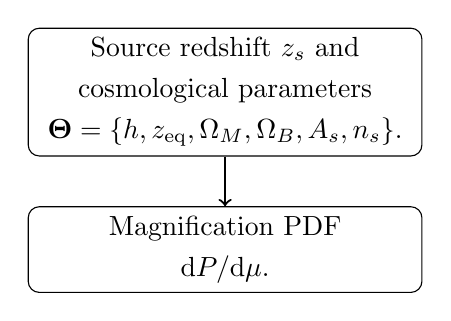
\begin{tikzpicture}[node distance=2.0cm]
\node[draw, rounded corners, align=center, minimum width=5.0cm] (input)
{Source redshift $z_s$ and \\[1mm]
cosmological parameters \\[1mm]
$\vect{\Theta} = \{h,z_{\rm eq},\Omega_M,\Omega_B,A_s,n_s\}$.};
\node[draw, rounded corners, align=center, minimum width=5.0cm, below of=input] (output)
{Magnification PDF \\[1mm]
$\mathrm{d}P/\mathrm{d}\mu$.};
\draw[->, thick] (input) -- (output);
\end{tikzpicture}
\end{center}

\B{The emulator is a conditional normalizing flow that models the smooth body of the distribution, combined with a power-law tail calibrated to the $\mu^{-2}$ asymptote of Sec.~\ref{sec:pdf}, a fitted low-magnification edge, and a flux-conservation calibration that enforces $\langle\mu^{-1}\rangle=1$ on the emulated distribution. Each component is trained on Monte Carlo realizations of the extended lens model, sampled over a wide prior on $\vect\Theta$ and $z_s$. The resulting emulator reproduces held-out simulations with a median Kullback-Leibler divergence of $0.0073$, comparable to the value $0.007$ reported for ACE-Lensing~\cite{Turker:2025rdt}, and recovers unbiased cosmological posteriors when used in place of the simulator in mock bright-siren Hubble-diagram reconstructions of the kind considered in Ref.~\cite{Vaskonen:2026ubd}.}

\begin{figure}
    \centering
    
\includegraphics[width=1.0\columnwidth]{plots/variance_D_L.pdf}
    \caption{The variance of luminosity distances induced by weak lensing.}
    \label{fig:variance_DL}
\end{figure}
\B{Figure~\ref{fig:variance_DL} shows the resulting variance of the luminosity
distance, $\sigma_{D_L}(z,\vect\Theta)$, across the cosmological parameter space.
Subhalos contribute a measurable fraction of this weak-lensing scatter. At
$z_s=5$ they raise $\langle\kappa^2\rangle$ by $\sim15\%$ over a smooth-halo-only
calculation, a contribution that standard-siren scatter budgets built from
smooth-halo simulations alone would miss.}

\section{Comparison with earlier works}
\label{sec:comparison}

\B{We first compare with ACE-Lensing~\cite{Turker:2025rdt}, a machine-learning
emulator of the magnification PDF trained on ray tracing through $N$-body
simulations. At the emulator level the two approaches reach comparable fidelity
to their respective training distributions, with a post-calibration median KL
divergence of $0.0073$ for our emulator against the value $0.007$ reported for
ACE-Lensing. At the model level, however, the predicted convergence fluctuations
differ. The (clipped, body-weighted) variance $\langle\kappa^2\rangle$ of our
simulation exceeds the ACE-Lensing prediction by $36$--$42\%$ at $z_s = 1$. This gap cannot
be attributed to the halo mass floor, since varying $M_{\rm min}$ over
$10^4$--$10^9\,\Msun$ moves $\langle\kappa^2\rangle$ in the wrong direction,
and the substructure contribution ($+15\%$ on $\langle\kappa^2\rangle$ at
$z_s = 5$), while significant, is smaller than the gap. We attribute the
difference primarily to the resolution limitations of $N$-body-based ray
tracing~\cite{DES:2025omh}.}

\B{At the population level we compare our subhalo model with
pyHalo~\cite{Gilman:2021sdr}. pyHalo generates substructure from an infall subhalo mass
function combined with per-object tidal evolution, anchored to observational
constraints on the projected substructure mass fraction, whereas we use the
evolved subhalo mass function of Ref.~\cite{Jiang:2014nsa} normalized by the
bound fraction $f_{\rm s}(N_\tau)$ anchored to the excursion-set formation
time. Despite the different construction, the resulting \emph{bound}-mass
functions agree well over the mass range relevant for lensing.
[Optionally include \texttt{plots/figures/pyhalo\_vs\_ours.png}; details in
\texttt{docs/subhalo/pyhalo\_pipeline\_comparison.md}.]}

\B{Finally, Ref.~[CITE-Mpetha-2402.19476] showed that the
$\sigma_{\ln\mu}(z)$ prescriptions currently used in bright standard siren
analyses are outdated and can underestimate the weak-lensing scatter. The
emulator presented here provides a drop-in replacement, $\sigma_{D_L}(z,
\vect\Theta)$ (Fig.~\ref{fig:variance_DL}), that consistently includes the
cosmology dependence and the subhalo contribution, which $N$-body-calibrated
fits cannot capture.}

\section{Conclusions}
\label{sec:conclusions}

\B{We have extended the stochastic weak-lensing model of Ref.~\cite{Vaskonen:2026ubd} to include the contribution of dark matter subhalos and an improved, correlated treatment of the clustering of field halos and filaments, and we have trained a fast machine-learning emulator that reproduces the resulting magnification probability distribution $dP/d\mu$ across the source redshift and a six-dimensional cosmological parameter space. The subhalo contribution is not negligible. At $z_s=5$ it raises $\langle\kappa^2\rangle$ by $\sim15\%$ over a smooth-halo-only calculation, a contribution that standard-siren scatter budgets built from smooth $N$-body halos alone would miss. The clustering of field halos on the scale probed here is a smaller, few-percent correction to the variance of $\ln\mu$, but we have shown how it depends on the assumed smoothing scale $R_s$, so it can be revisited as external constraints on the relevant scale improve. The resulting emulator matches the accuracy of existing machine-learning emulators of the magnification distribution while incorporating this extended physical model, at a fraction of the computational cost of the underlying Monte Carlo, making likelihood-based inference of the kind considered in Ref.~\cite{Vaskonen:2026ubd} practical for the extended model.}

\B{Several simplifications remain. The concentration-mass relation and ellipticity distribution of field halos are calibrated on the halo, rather than the subhalo, population. Subhalos are modeled as untruncated NFW profiles rather than tidally truncated ones. The projected shear of every lens is summed with a single polar angle rather than its full spin-2 transformation, an approximation we have checked affects $\langle\gamma^2\rangle$ at only the $\sim0.5\%$ level. None of these is expected to qualitatively change our conclusions, but a more refined treatment, benchmarked directly against $N$-body simulations with sufficient mass resolution to resolve substructure, would be a natural next step, as would extending the comparison with $N$-body-based emulators such as ACE-Lensing~\cite{Turker:2025rdt} beyond the halo-only level considered here.}

\B{Looking ahead, the accuracy and speed of the emulator presented here make it a practical drop-in replacement for the smooth-halo lensing-scatter prescriptions currently used in bright-siren forecasts and analyses~\cite{CITE-Mpetha}, and open the possibility of extending the cosmological reach of bright-siren weak lensing beyond $\sigma_8$ alone. Since the abundance and internal structure of dark matter halos and subhalos depend on the nature of dark matter, applying a similar analysis to warm, fuzzy, or self-interacting dark matter scenarios could turn the weak-lensing scatter of bright sirens into a probe of small-scale structure complementary to galactic and Lyman-$\alpha$ constraints.}

\section*{Acknowledgments}

This work was supported by the Estonian Research Council grants TARISTU24-TK3 and TARISTU24-TK10, and the Center of Excellence program TK202 of the Estonian Ministry of Education and Research.

\bibliography{refs}

% ============================================================================
% \B{NOTES FOR THE REVISION (delete before submission)}
%
% New refs.bib entries needed (pull from Inspire):
%   Sheth:1999mn     - Sheth & Tormen 1999, MNRAS 308, 119 (PBS bias)
%   Sheth:1999su     - Sheth, Mo & Tormen 2001 (ellipsoidal collapse HMF)
%   Dutton:2014xda   - Dutton & Maccio 2014, arXiv:1402.7073 (c200(M,z))
%   Allgood:2005eu   - Allgood et al. 2006 (halo shapes)
%   Wright:1999tv    - Wright & Brainerd 2000 (NFW lensing functions)
%   Yan:2011ux       - Yan & Fan 2011, ApJ 730, 33, arXiv:1101.3847 (filaments)
%   Bryan:1997dn     - Bryan & Norman 1998 (Delta_vir fit)
%   Giocoli:2006yz   - Giocoli, Moreno, Sheth & Tormen 2007, MNRAS 376, 977
%                      (alpha_f formula; replaces Giocoli:2011hz at that spot)
%   Green:2021       - Green, van den Bosch & Jiang 2021, arXiv:2103.01227
%                      (radial bias fit) -- REPLACE with the exact Inspire key
%   Klypin:2010qw    - Klypin, Trujillo-Gomez & Primack 2011, arXiv:1002.3660
%                      (Bolshoi)
%   Springel:2008cc  - Springel et al. 2008, arXiv:0809.0898 (Aquarius A-1
%                      Einasto subhalo density) -- RESOLVED 2026-07-23, key found
%                      in paper_prod/production.tex (user's Overleaf copy)
%   Han:2015pua      - Han, Cole, Frenk & Jing 2016, arXiv:1509.02175 (radial
%                      bias power law x^1.3, Aquarius A) -- RESOLVED 2026-07-23,
%                      ditto (found in production.tex)
%   Zacharegkas:2026zzy - Zacharegkas et al. 2026, arXiv:2607.10419 (Diffhalos
%                      concentration-conditioned SHMF) -- RESOLVED 2026-07-23,
%                      ditto (production.tex uses the zzy suffix)
%   Gilman:2021sdr   - pyHalo (Gilman et al.) -- RESOLVED 2026-07-23, ditto
%   CITE-Mpetha      - Mpetha, Congedo & Taylor 2024, PRD 110, 023502,
%                      arXiv:2402.19476 -- key TBD (still unresolved in
%                      production.tex too -- Comparison section there is only
%                      an outline, not yet written)
%
% Figure files (copy to Overleaf plots/):
%   plots/fig_clustering_field.pdf          (new, generated 2026-07-20)
%   plots/fig_subhalo_population.pdf        (new, generated 2026-07-20)
%   plots/sigma_partition_vs_kthr_bias.pdf  (repo path:
%       paper_prod/plots/figures/sigma_partition_vs_kthr_bias.pdf -- replaces
%       the legacy shot-only plots/sigma_partition_vs_kthr.pdf)
%   plots/fig_magnification_pdf_zs.pdf          (Sec. II.B; generator
%       paper_prod/scripts/plot_fig_magnification_pdf.py -> figures/, run guide
%       paper_prod/scripts/README_magnification_pdf.md; MC run by user)
%   plots/fig_magnification_pdf_ingredients.pdf (ditto; baseline/+subhalos/+clustering
%       at z_s=5)
%   plots/fig_subhalo_sigma_decomposition_{mean,scatter}.pdf  (repo path:
%       paper_prod/plots/figures/fig_subhalo_sigma_decomposition_{mean,scatter}.pdf --
%       host/subhalo convergence + scatter decomposition for subhalo_model=4, split
%       2026-07-23 into two single-panel figures (was one two-panel figure); REPLACES
%       the obsolete eps_sub partition figure sigma_partition_vs_subhalo_factor.png,
%       dropped 2026-07-23 with the kappa_u / unresolved apparatus)
%
% Clustering window/scale (updated 2026-07-20, user decision):
%   - Window = spherical 3D top-hat (bias_window=1), replacing the transverse
%     disk. Isotropic smoothing, gives sigma^2_1D = sigma^2(R_s); mode cutoff
%     N_max = L/R_s now immaterial (top-hat suppresses the power there).
%   - R_s = 20 Mpc default (user, 2026-07-20), NOT R_L(1e14)=8.44 Mpc: R_L is a
%     Lagrangian radius, not a smoothing scale. Consequence: top-hat point-field
%     sigma 0.972 (8.44 Mpc) -> 0.530 (20 Mpc), i.e. clustering variance ~30%;
%     clustering becomes a conservative small correction. R_s = 20 Mpc is the
%     SETTLED paper value (Gala, decision made 2026-07-23); it reverses the
%     2026-07-16 8.44 Mpc default, which is kept only as the signal-weighted
%     comparison curve in Fig. clustering.
%   - Gaussian window (bias_window=2) is a shape-robustness option; matched
%     radius R_G = 9.4 Mpc at R_s=20 Mpc.
%   - CODE DEFAULT NOT FLIPPED: shipped default stays bias_model=0 (legacy);
%     production config bias_model=1, bias_window=1, bias_Rperp=20000 is passed
%     explicitly pending Ville's sign-off. See docs/bias_window_design_plan.md,
%     data/results/bias_window/report.md.
%   - 20 Mpc MC DONE (data/results/bias_window/rs_dependence.md): the full config
%     (bias_weak on) gives Var_clip(lnmu)/no-clustering = 1.15/1.11/1.08 at
%     z_s = 0.5/1/5, i.e. +8-15% -- NOT "few percent". TODO: reconcile the
%     Conclusions wording ("smaller, few-percent correction") with these numbers.
%
% Other open decisions flagged in blue:
%   - Filament clustering bias: RESOLVED 2026-07-23 -- switched to the
%     PBS filament-barrier bias b_F(M,z) (10-20% lower than the halo bias),
%     implemented as fil_bias in the code (docs/filament_bias_note.md).
%
% 2026-07-23b -- structural sections drafted (Abstract, Introduction, Sec. II.B
% Magnification PDF, ML methodology paragraph, Conclusions), all new text in
% \B{}. Style calibrated against papers/core/Vaskonen_2026_GWWeakLensingSigma8.pdf
% (the companion/predecessor paper, Vaskonen:2026ubd). Notes:
%   - Added \label{sec:lensing,pdf,ml,comparison,conclusions} for the new
%     Sec. I outline paragraph's \ref{}s -- check these don't collide with
%     labels already in production.tex if merging by hand.
%   - Sec. II.B text states the (already-verified) mu^-2 image-plane tail and
%     the flux-conservation check qualitatively; no new figure -- Vaskonen's
%     own paper doesn't plot dP/dmu shape directly either (only sigma_DL(z)
%     and the lens-PDF-of-r,M figure), so this matches precedent.
%   - [CITE-caustic-scaling]: deliberately left unresolved. The mu^-2/mu^-3
%     image/source-plane duality is verified IN THIS REPO (docs/
%     edge_tail_flux_note.md, Hill-alpha fit 1.95-2.03 on 10M samples), but I
%     do not have a reliable specific literature citation for the generic
%     fold-caustic p(mu)~mu^-3 result on hand -- do not fill this with a guess;
%     Vaskonen likely knows the right ref (textbook caustic-theory result,
%     e.g. Schneider/Ehlers/Falco or a magnification-pdf-tail paper).
%   - Conclusions cites \cite{CITE-Mpetha} (same placeholder key as the
%     Comparison section -- resolve together) and closes with a
%     dark-matter-probe outlook paragraph modeled on Vaskonen 2026's own
%     closing paragraph (warm/fuzzy/compact DM) -- verify this framing before
%     keeping it; it is a genuine extrapolation beyond what this repo has
%     tested, not a verified code-backed claim like the rest of the draft.
%   - ML section KL=0.0073 / ACE 0.007 comparison reuses the number already
%     used in Sec. IV (G3 in draft_comments_memo.md) -- kept consistent
%     rather than re-derived.
%   - NOT touched: production.tex (per standing rule). These sections are
%     currently pure placeholders there ("...", elided intro, no Sec. II.B
%     text, empty Conclusions) -- propose importing after Ville reads.
%   - Radial-profile fit variant: Green+21 transition fit (0.54, 5/2) adopted;
%     direct Bolshoi fit would be (0.94, 2.52) (stronger depletion).
%
% 2026-07-23c status (Gala):
%   - R_s DECIDED = 20 Mpc (settled paper value; see clustering note above).
%   - Sec. IV Comparison with earlier works: content to be FINALIZED AFTER the ML
%     training results are in -- treat the current \B{} comparison text as
%     provisional until then.
% ============================================================================

\end{document}
